% Created by tikzDevice version 0.12.3 on 2020-06-17 00:27:50
% !TEX encoding = UTF-8 Unicode
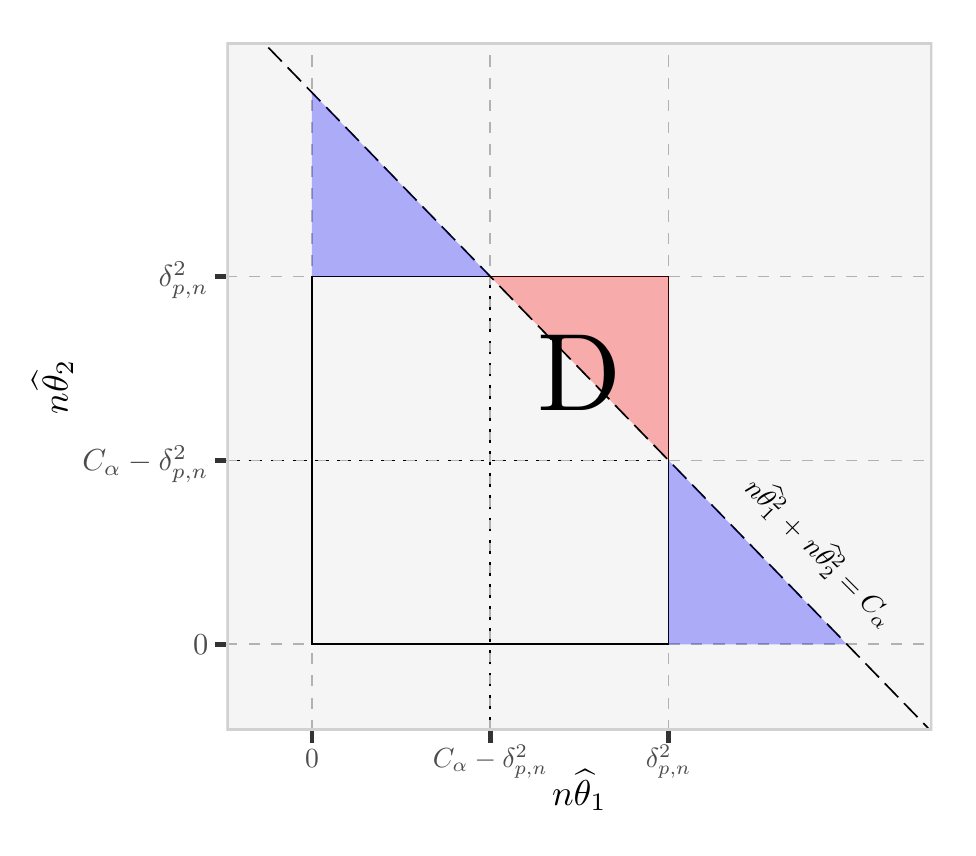
\begin{tikzpicture}[x=1pt,y=1pt]
\definecolor{fillColor}{RGB}{255,255,255}
\path[use as bounding box,fill=fillColor,fill opacity=0.00] (0,0) rectangle (332.44,289.08);
\begin{scope}
\path[clip] (  0.00,  0.00) rectangle (332.44,289.08);
\definecolor{drawColor}{RGB}{255,255,255}
\definecolor{fillColor}{RGB}{255,255,255}

\path[draw=drawColor,line width= 0.6pt,line join=round,line cap=round,fill=fillColor] (  0.00,  0.00) rectangle (332.44,289.08);
\end{scope}
\begin{scope}
\path[clip] ( 71.80, 35.03) rectangle (326.94,283.58);
\definecolor{fillColor}{gray}{0.96}

\path[fill=fillColor] ( 71.80, 35.03) rectangle (326.94,283.58);
\definecolor{drawColor}{gray}{0.70}

\path[draw=drawColor,line width= 0.6pt,dash pattern=on 4pt off 4pt ,line join=round] ( 71.80, 66.26) --
	(326.94, 66.26);

\path[draw=drawColor,line width= 0.6pt,dash pattern=on 4pt off 4pt ,line join=round] ( 71.80,132.72) --
	(326.94,132.72);

\path[draw=drawColor,line width= 0.6pt,dash pattern=on 4pt off 4pt ,line join=round] ( 71.80,199.18) --
	(326.94,199.18);

\path[draw=drawColor,line width= 0.6pt,dash pattern=on 4pt off 4pt ,line join=round] (102.72, 35.03) --
	(102.72,283.58);

\path[draw=drawColor,line width= 0.6pt,dash pattern=on 4pt off 4pt ,line join=round] (167.15, 35.03) --
	(167.15,283.58);

\path[draw=drawColor,line width= 0.6pt,dash pattern=on 4pt off 4pt ,line join=round] (231.58, 35.03) --
	(231.58,283.58);
\definecolor{drawColor}{RGB}{0,0,0}

\path[draw=drawColor,line width= 0.6pt,line cap=rect] (102.72, 66.26) rectangle (231.58,199.18);
\definecolor{fillColor}{RGB}{255,0,0}

\path[fill=fillColor,fill opacity=0.30] (167.15,199.18) --
	(231.58,199.18) --
	(231.58,132.72) --
	cycle;

\path[draw=drawColor,line width= 0.6pt,dash pattern=on 7pt off 3pt ,line join=round] ( 80.00,289.08) -- (326.94, 34.37);

\node[text=drawColor,rotate=-45.00,anchor=base,inner sep=0pt, outer sep=0pt, scale=  1.00] at (283.93, 97.07) {$n \widehat{\theta}^2_1$ + $n \widehat{\theta}^2_2 = C_{\alpha}$};
\definecolor{fillColor}{RGB}{0,0,255}

\path[fill=fillColor,fill opacity=0.30] (102.72,199.18) --
	(102.72,265.64) --
	(167.15,199.18) --
	cycle;

\path[fill=fillColor,fill opacity=0.30] (231.58,132.72) --
	(296.02, 66.26) --
	(231.58, 66.26) --
	cycle;

\path[draw=drawColor,line width= 0.6pt,dash pattern=on 1pt off 3pt ,line join=round] ( 71.80,132.72) --
	(231.58,132.72);

\path[draw=drawColor,line width= 0.6pt,dash pattern=on 1pt off 3pt ,line join=round] (167.15, 35.03) --
	(167.15,199.18);

\node[text=drawColor,anchor=base,inner sep=0pt, outer sep=0pt, scale=  3.98] at (199.37,150.91) {D};
\definecolor{drawColor}{gray}{0.82}

\path[draw=drawColor,line width= 1.7pt,line join=round,line cap=round] ( 71.80, 35.03) rectangle (326.94,283.58);
\end{scope}
\begin{scope}
\path[clip] (  0.00,  0.00) rectangle (332.44,289.08);
\definecolor{drawColor}{gray}{0.30}

\node[text=drawColor,anchor=base east,inner sep=0pt, outer sep=0pt, scale=  1.10] at ( 65.33, 62.48) {0};

\node[text=drawColor,anchor=base east,inner sep=0pt, outer sep=0pt, scale=  1.10] at ( 65.33,128.93) {$C_{\alpha} - \delta_{p,n}^2$};

\node[text=drawColor,anchor=base east,inner sep=0pt, outer sep=0pt, scale=  1.10] at ( 65.33,195.39) {$\delta_{p,n}^2$};
\end{scope}
\begin{scope}
\path[clip] (  0.00,  0.00) rectangle (332.44,289.08);
\definecolor{drawColor}{gray}{0.20}

\path[draw=drawColor,line width= 1.7pt,line join=round] ( 67.53, 66.26) --
	( 71.80, 66.26);

\path[draw=drawColor,line width= 1.7pt,line join=round] ( 67.53,132.72) --
	( 71.80,132.72);

\path[draw=drawColor,line width= 1.7pt,line join=round] ( 67.53,199.18) --
	( 71.80,199.18);
\end{scope}
\begin{scope}
\path[clip] (  0.00,  0.00) rectangle (332.44,289.08);
\definecolor{drawColor}{gray}{0.20}

\path[draw=drawColor,line width= 1.7pt,line join=round] (102.72, 30.76) --
	(102.72, 35.03);

\path[draw=drawColor,line width= 1.7pt,line join=round] (167.15, 30.76) --
	(167.15, 35.03);

\path[draw=drawColor,line width= 1.7pt,line join=round] (231.58, 30.76) --
	(231.58, 35.03);
\end{scope}
\begin{scope}
\path[clip] (  0.00,  0.00) rectangle (332.44,289.08);
\definecolor{drawColor}{gray}{0.30}

\node[text=drawColor,anchor=base,inner sep=0pt, outer sep=0pt, scale=  1.00] at (102.72, 21.67) {0};

\node[text=drawColor,anchor=base,inner sep=0pt, outer sep=0pt, scale=  1.00] at (167.15, 21.67) {$C_{\alpha} - \delta_{p,n}^2$};

\node[text=drawColor,anchor=base,inner sep=0pt, outer sep=0pt, scale=  1.00] at (231.58, 21.67) {$\delta_{p,n}^2$};
\end{scope}
\begin{scope}
\path[clip] (  0.00,  0.00) rectangle (332.44,289.08);
\definecolor{drawColor}{RGB}{0,0,0}

\node[text=drawColor,anchor=base,inner sep=0pt, outer sep=0pt, scale=  1.30] at (199.37,  8.03) {$n \widehat{\theta}_1$};
\end{scope}
\begin{scope}
\path[clip] (  0.00,  0.00) rectangle (332.44,289.08);
\definecolor{drawColor}{RGB}{0,0,0}

\node[text=drawColor,rotate= 90.00,anchor=base,inner sep=0pt, outer sep=0pt, scale=  1.30] at ( 14.45,159.30) {$n \widehat{\theta}_2$};
\end{scope}
\end{tikzpicture}
